\documentclass{report} 
\usepackage{amsmath} 
\usepackage{graphicx} 

\begin{document}
\title{Homework 5 report}
\author{Jun Cheng}
\maketitle

\section*{Problem 1} 
\subsection*{Part (a)} 
Buy-and-hold strategy: 

Rebalancing strategy: 
Parameters: 
\begin{itemize}
\item $S_0$: initial stock price.
\item $S_t$: stock price at time $t$.
\item $x_t$: number of stock shares at time $t$.
\item $C_t$: cash held at time $t$ in dollar. 
\end{itemize}
Use the Monte Carlo to simulate the stock price to get all $S_t$,  and then update all all $C_i $ and $x_i$: 
\begin{align*}
&C_{t+1}=\frac{x_tS_{t+1}}{2} \\
&x_{t+1}=\frac{C_1}{S_1}\\
\end{align*}
Monte Carlo simulations: 
\begin{itemize}
\item $ u=2$
\item $ d=0.5$
\item $p_u = p_d = 0.5$
\end{itemize} 
Running the attached code, we can get, 
\begin{align*}\begin{array}{ll}
E(U)=56.7275  & var(U) =171812\\
E(V)=  8.76893 & var(V)=366.343\\
\end{array} \end{align*}
To get $95\% $ confidence interval, we should $\delta = 0.05$, $z_{1-\delta/2}=1.96$, then the confidence interval
\begin{align*}
\begin{array}{ll}
\left[E(U)-1.96\frac{\sigma_u}{\sqrt{n}}, E(U)+1.96\frac{\sigma_u}{\sqrt{n}}\right]  :   [41.8947, 71.5603]\\
\left[E(V)-1.96\frac{\sigma_v}{\sqrt{n}},  E(V)+1.96\frac{\sigma_v}{\sqrt{n}}\right]  :   [ 8.08401, 9.45385  ]\\
\end{array}
\end{align*}

\subsection*{Part (b)}
Now we have new random variable $ T=V-U $.  Since $V$ and $U$ are independent, then we can have
\begin{align*}
& E(T) = E(V)-E(U) = -47.9586 \\
& var(T) = var(T)+var(E) = 172178\\
\end{align*}
then the confidence interval  
$$\left[E(T)-1.96\frac{\sigma_u}{\sqrt{n}}, E(T)+1.96\frac{\sigma_u}{\sqrt{n}}\right]  :   [ -62.8071, -33.11 ]\\ $$
 
\subsection*{Part(c)} 
If we use the same stream of random numbers then the confidence interval is
\begin{align*}
& E(V-U) =-37.2872 \\
& var(V-U) = 125996\\
& Confidence interval :  [-49.9892, -24.5851 ] \\
\end{align*}
This confidence is wider than that of Part(b). Because when we use the same stream of random numbers to simulate both $U$ and $V$, we need to consider about the correlation between them. Obviously $U$ and $V$ are positively correlated. This is kind of variate control method which can reduce the variance of Monte Carlo simulation. 

\subsection*{Part(d)} 
If we use the same stream of random numbers then the confidence interval is
\begin{align*}
& E(log_{10}V-log_{10}U) = 0.491468\\
& var(log_{10}V-log_{10}U) = 0.439653\\
& Confidence interval :  [ 0.46774, 0.515195] \\
\end{align*}
Compare with Part(c) using utility functions gives a better quatitative comparison of investment alternatives, because the variance range is narrow and then it is more easy to quantify the risk. 

\newpage
\section*{Problem 2}
\subsection*{Part(a)} 
For daily rebalancing:  $$ E(error) = -0.0056658$$
$$ var(error) = 0.272379 $$
$$ \sigma = 0.52 $$
For weekly rebalancing:: $$ E(error) = -0.02113$$
$$ var(error) =1.88433 $$
$$ \sigma = 1.37$$
\begin{figure} \centering
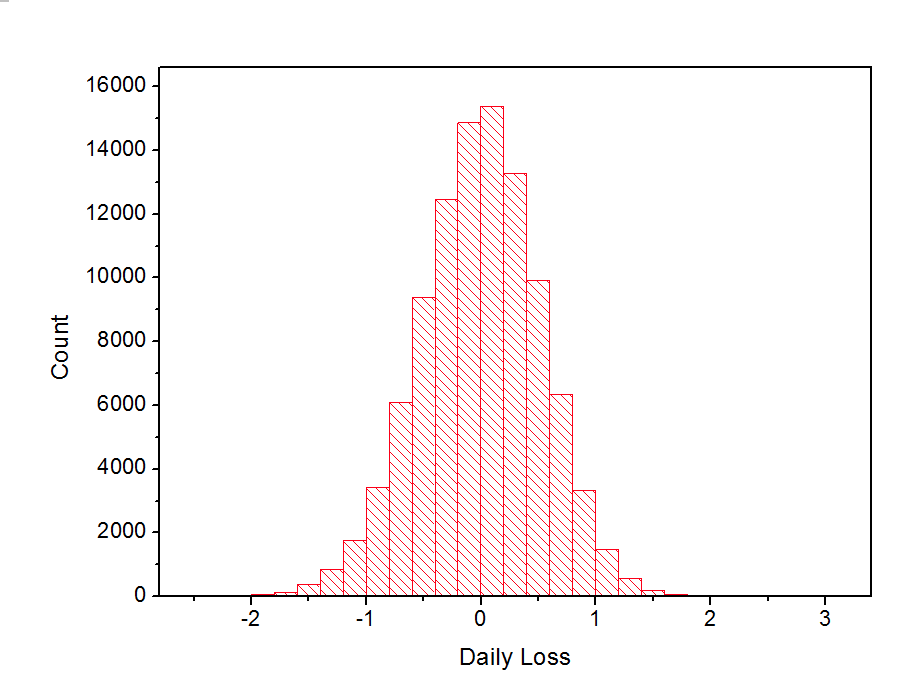
\includegraphics[width=\textwidth]{daily}
\caption{Delta hedging loss for daily reblancing}  

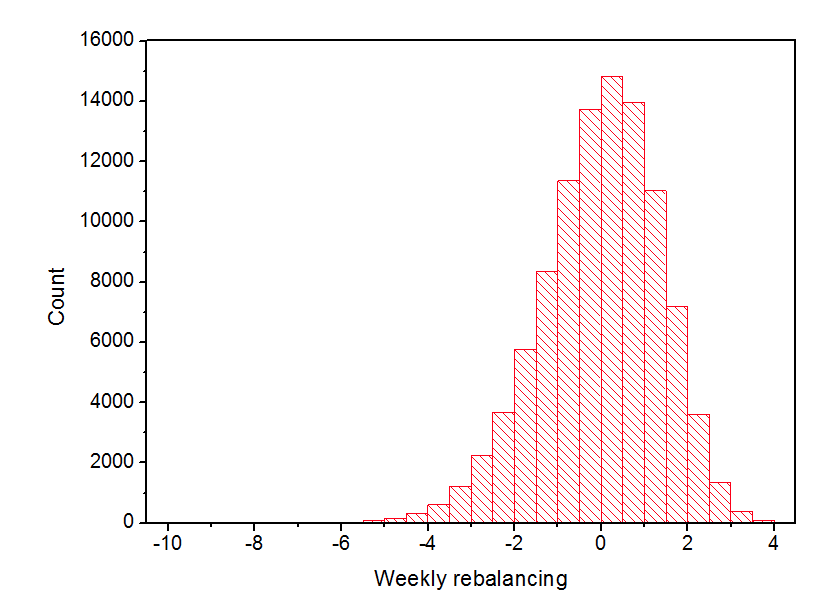
\includegraphics[width=\textwidth]{weekly}
\caption{Delta hedging loss for weekly reblancing}  
\end{figure}

\subsection*{Part(b)} 
Changing values of $\mu$ doesn't change the result. That makes sense because the value of the option and the delta both are not related to $\mu$. 

\subsection*{Part(c)} 
Yes, the hedging error is $O((\Delta T)^\alpha)$. 
\begin{align*}\begin{array}{ll}
dt & abs(error)  \\
 1e-06 &  7.17567e-05\\
1e-05  &	0.000637571\\
0.0001&	0.000753965\\
0.001&	0.00321909\\
0.01	&    0.0187996\\
\end{array}\end{align*}
\begin{figure}
\caption{Plot of $log(error)$  vs  $log(dt) $ }
\label{fig:log}
\centering
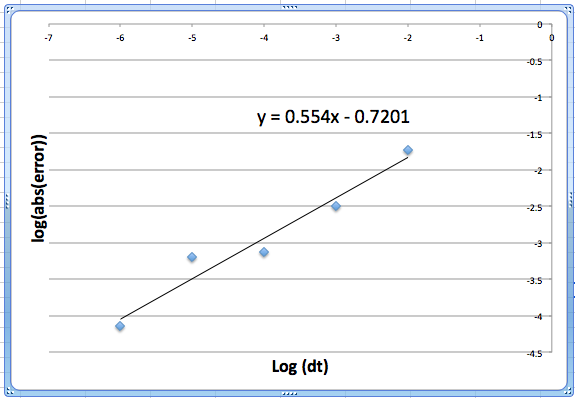
\includegraphics[width=\textwidth]{log_dt}
\end{figure}
The linear regression equation is:  $ y=0.554x-0.7201$. Therefore, the $\alpha$ is 0.554 as show in Figure \ref{fig:log}. \\

\subsection*{Stop-loss strategy} 
For daily rebalancing:  $$ E(error) = 0.947117$$
$$ var(error) = 37.2515 $$
$$ \sigma = 6.103 $$
For weekly rebalancing:: $$ E(error) = 0.91152$$
$$ var(error) =35.9063 $$
$$ \sigma = 5.992$$
\begin{figure} \centering
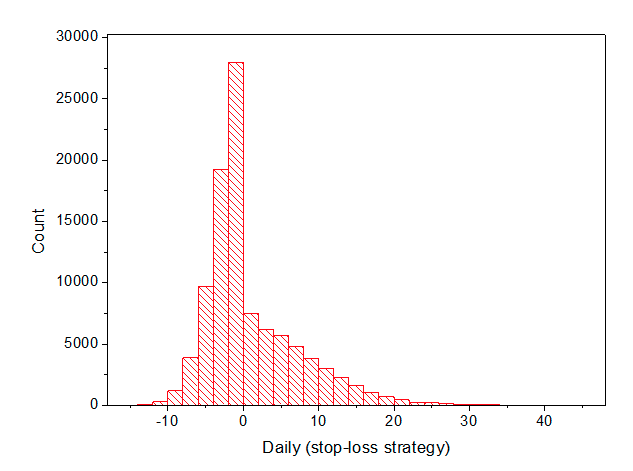
\includegraphics[width=\textwidth]{Daily_b}\label{Daily_b}
\caption{Stop-loss strategy loss for daily reblancing}  
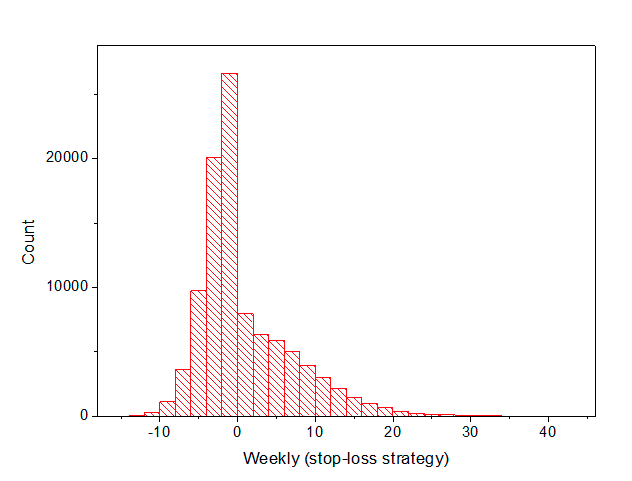
\includegraphics[width=\textwidth]{Weekly_b}\label{Weekly_b}
\caption{Stop-loss strategy loss for weekly reblancing}  
\end{figure}
Compared with delta hedging, you don't need to frequently buy or sell underlying as delta hedging.  But disadvantage is that this method introduce large variance for the final loss/gain, which is shown in Figure\ref{Daily_b} and Figure \ref{Weekly_b}. 

	
\newpage
\section*{Problem 3}
\subsection*{Part(a)} 
\begin{align*} 
&E(X)= 7.23497\\
&std(X)= 7.9105\\
&95\% confidence interval: 0.0310091\\
\end{align*}
I used 1million replications to get this 95\% interval.  This estimator has bias, which is  than real value. 

\subsection*{Part(b)}
\begin{align*} 
&E(X)= 7.22314\\
&std(X)= 6.43481\\
&95\% confidence interval: 0.0252244\\
\end{align*}
This is an unbiased estimator of UOP option. The standard deviation is smaller. 

\newpage
\section*{Problem 4} 
\subsection*{Part(a)}
Implementation of Cholesky algorithm: 
\begin{align*}\begin{array}{l}
a_{i,j}=(\sum_{i,j}-\sum_{k=1}^{j-1}a_{i,k}a_{j,k})/a_{i,j}, j<i\\
a_{i,i}=\sqrt{\sum_{i,i}-\sum_{k=1}^{i-1}a_{i,k}^2}\\
\end{array}\end{align*} 
Parameters setting: 
\begin{itemize} 
\item Number of steps: 100
\item Number of replication: 30000
\item ====================
\item Price of the option: \em \textbf{58.53}
\end{itemize}
\subsection*{Part(b)}
The convergence of Monte Carlo estimate is slow, which is $\frac{1}{\sqrt{n}} $.

\subsection*{Part(c)}
Take Euler Scheme for example, for one stock: 
\begin{align*} 
S_T^i=S_0^iexp\left(\left(r-\frac{1}{2}\sigma^2\right)dt+\sigma\sqrt{dt}\sum_{t=1}^{T}Z_t^i\right)\\
\end{align*}
Then: 
\begin{align*}
d(S_T^1...S_T^d)^{1/d}=dS_0^iexp\left(\left(r-\frac{1}{2}\sigma^2\right)T+\frac{\sigma\sqrt{dt}}{d}\sum_{t=1}^{T}\sum_{i=1}^{d}Z_t^i\right)\\
\end{align*}
And then the expectation of $\left(d(S_T^1...S_T^d)^{1/d}-K\right)^+$ is known using Block Schole formula. 
Also, we know that  $\left(d(S_T^1...S_T^d)^{1/d}-K\right)^+$ is correlated with $\left(S_T^1+...+S_T-K\right)^+$. Therefore, we can use it as a control variate to reduce the variance. 

\subsection*{Part(d)} 
$$ var(\sum_{i=1}^{d}Z_i)  = 10 + 90*\rho_{ij}\sigma_i\sigma_j=37 $$ 
The option with payoff function $\left(d(S_T^1...S_T^d)^{1/d}-K\right)^+$ has this feature: \\
\begin{itemize} 
\item Stock price at time 0:  $dS_0=1000$\\
\item Maturity time: $T=1$ \\
\item Adjusted sigma: $\sigma_{new}= \frac{\sqrt{37}\sigma_{old}}{d} = 0.091 $
\item Adjusted risk free rate: $r=r_{old}-\frac{\sigma_{old}^2}{2}+\frac{\sigma_{new}^2}{2}= 0.03 $
\item Strike price:  $ K = 1000 $
\end{itemize}

Using the Black Schole formula, we can have the expected value:  $52.45 $

The optimal b is : 
$$b^*=\frac{\sum_{i=1}^{n}(X_i-\hat{X}) (Y_i-\hat{Y}) }{\sum_{i=1}^{n}(X_i-\hat{X})^2} = 1.037 $$
Then the new payoff function becomes: 
$$\hat{Y_n}=\frac{1}{n}\sum_{i=1}^{n}(Y_i-b(X_i-E(X))), $$

\begin{figure} \centering
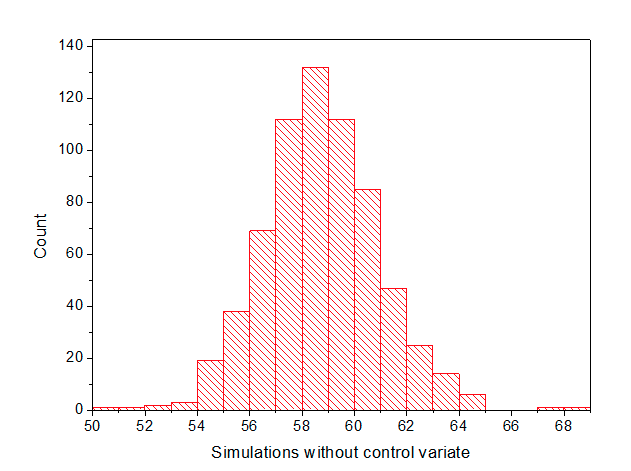
\includegraphics[width=\textwidth]{before}\label{fig:before}
\caption{Histgram for the naive Monte Carlo simulation of the price. The variance is relatively large.}  
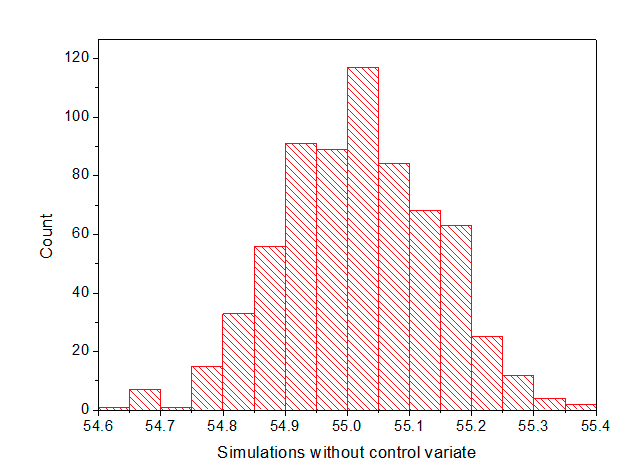
\includegraphics[width=\textwidth]{after}\label{fig:after}
\caption{Histgram for the Monte Carlo simulation of the price using control variate to reduce the variance. The variance is relatively small.}  
\end{figure}
The implementation is attached. And we can conclude that the variance is reduced which is shown in Figure \ref{fig:before} and Figure \ref{fig:after}. 

\end{document}